\documentclass[12pt]{report}

% Font and text formatting packages
\usepackage{microtype} % Improved text alignment and spacing
\usepackage[bitstream-charter]{mathdesign}
\usepackage{XCharter} % XCharter font
\usepackage[scaled]{beramono} % Monospaced font styling
% \usepackage[italic]{mathastext} % Italicizes math in text font for consistency

% Conditional checking
\usepackage{etoolbox}

% Enhanced typography
\usepackage[normalem]{ulem} % Underlining
\usepackage{contour} % Outline text (used with \contour command)
\usepackage{xpatch} % Enables patching commmands for typographical modifications
\usepackage{bm} % Italic bold

% Scientific notation and chemical formulas
\usepackage[version=4]{mhchem} % For chemical notation
\usepackage{siunitx} % Consistent handling of units

% Graphics
\usepackage{graphicx} % Essential for including images
\usepackage{subcaption} % Subfigures and subcaptions
\graphicspath{{./images/}} % Path for images directory

% Document layout
\usepackage[margin=1in]{geometry} % 1-inch margins
\usepackage{multicol} % Multi-column layouts

% Custom captions formatting
\usepackage{caption}
\DeclareCaptionFormat{custom}{\textbf{#1.} #3}
\captionsetup{format=custom}


\usepackage{csquotes} % Recommended for quotes in citations
\usepackage[style=apa, backend=biber]{biblatex} % APA style citations
\addbibresource{references.bib} % Reference file


% Custom underlining with contour effect
\contourlength{1.7pt} % Default contour length
\NewDocumentCommand{\ul}{O{2.62pt} O{0.45pt} O{1.5pt} m}{%
  \begingroup%
  \renewcommand\ULdepth{#1}%
  \renewcommand\ULthickness{#2}%
  \contourlength{#3}%
  \uline{\phantom{#4}}\llap{\contour*{white}{#4}}%
  \endgroup%
}

% Additional custom commands
\def\code#1{\texttt{#1}} % Inline code styling
\newcommand{\goldenRatio}{1.6180} % Golden ratio constant
\newcommand{\inverseGoldenRatio}{0.6180} % Inverse golden ratio constant

% Define automatic kerning for footnotes next to punctuation
\makeatletter
\xpatchcmd{\@makefnmark}{\hss}{\kern-0.5em\hss}{}{}
\makeatother

% Automatic extra spacing around em-dashes
\xpretocmd{\textemdash}{\hspace{0.1em}}{}{}
\xapptocmd{\textemdash}{\hspace{0.1em}}{}{}

\title{\textbf{Pulsed Nuclear Magnetic Resonance} \\\vspace{-0.6cm}}
\date{
    November 8, 2024 \\\vspace{0.5cm}
    \large{\textsc{Modern Physics Lab}}
}
\author{
    \ul{Micah Hillman} \and Cordney Nash
}

\begin{document}
\maketitle

\section*{Introduction}
{
    Pulsed nuclear magnetic resonance (\textsc{pnmr}) is a method for probing the dynamics of small-scale structures like molecules and nuclei using radiofrequency (\textsc{rf}) energy pulses in the presence of a constant, strong magnetic field, $\bm{B}_0 \parallel \hat{\mathrm{z}}$. Protons in certain nonpolar samples can be aligned along $\bm{B}_0$ and subjected to \textsc{rf} pulses that transiently alter their alignment, rotating their spins into the $\hat{\mathrm{x}}$–$\hat{\mathrm{y}}$ plane, where they begin to precess around an effective magnetic field, $\bm{B}_1$. This precession induces a voltage in a receiver solenoid that detects the oscillating induced magnetic field in the $\hat{\mathrm{x}}$–$\hat{\mathrm{y}}$ plane. Over time, the magnetization vector relaxes back to its equilibrium state along $\bm{B}_0$ through two primary energy-transfer mechanisms: \textbf{spin–lattice relaxation}—where energy is transferred to the molecular lattice—and \textbf{spin–spin relaxation}—where energy is exchanged among the spins of other nuclei. Both of these pathways have associated characteristic timescales called ``relaxation times'' ($T_1$ and $T_2$, respectively); in this experiment, we used a TeachSpin\textsuperscript{\tiny\textregistered} \textsc{nmr} apparatus to measure $T_1$ and $T_2$ for both glycerin and mineral oil samples.
}

\section*{Theory}
{
    The intrinsic spin of a proton generates a magnetic moment $\bm{\mu}$ which interacts with external magnetic fields. When a magnetic field $\bm{B}_0$ is applied, the magnetic moments of the protons tend to align with $\bm{B}_0 \parallel \hat{\mathrm{z}}$, minimizing their potential energy. With orthogonal \textsc{rf} pulses, we can rotate their spins into the $\hat{\mathrm{x}}$–$\hat{\mathrm{y}}$ plane, initiating a precession around $\bm{B}_1$, the effective magnetic field due to the \textsc{rf} pulses. The angle of this rotation, known as the \ul{flip angle}, can be modulated by the duration and amplitude of the \textsc{rf} pulse. When the pulse frequency matches the \ul{Larmor frequency},\footnote{The natural frequency of the proton's precession.} the spins resonate, rotating away from their equilibrium alignment with $\bm{B}_0$. The duration of the \textsc{rf} pulse determines how far the spins rotate, allowing for the accurate manipulation of spin dynamics essential for \textsc{pnmr} experiments.

    The behavior of the resonance in both spin–lattice (\ref{eq:1}) and spin–spin (\ref{eq:2}) relaxation can be described as functions of the \ul{pulse interval}\footnote{The time interval between consecutive \textsc{rf} pulses.} $\Delta t$:
    \begin{equation}
        V = V_{0} \left( 1 - 2e^{-\Delta t/T_{1}} \right)\!,
        \label{eq:1}
    \end{equation}
    \begin{equation}
        V = V_{0} \left( e^{-\Delta t / T_{2}} \right)\!,
        \label{eq:2}
    \end{equation}
}

\section*{Methods}
{
    \begin{figure}[tbh]
        \centering
        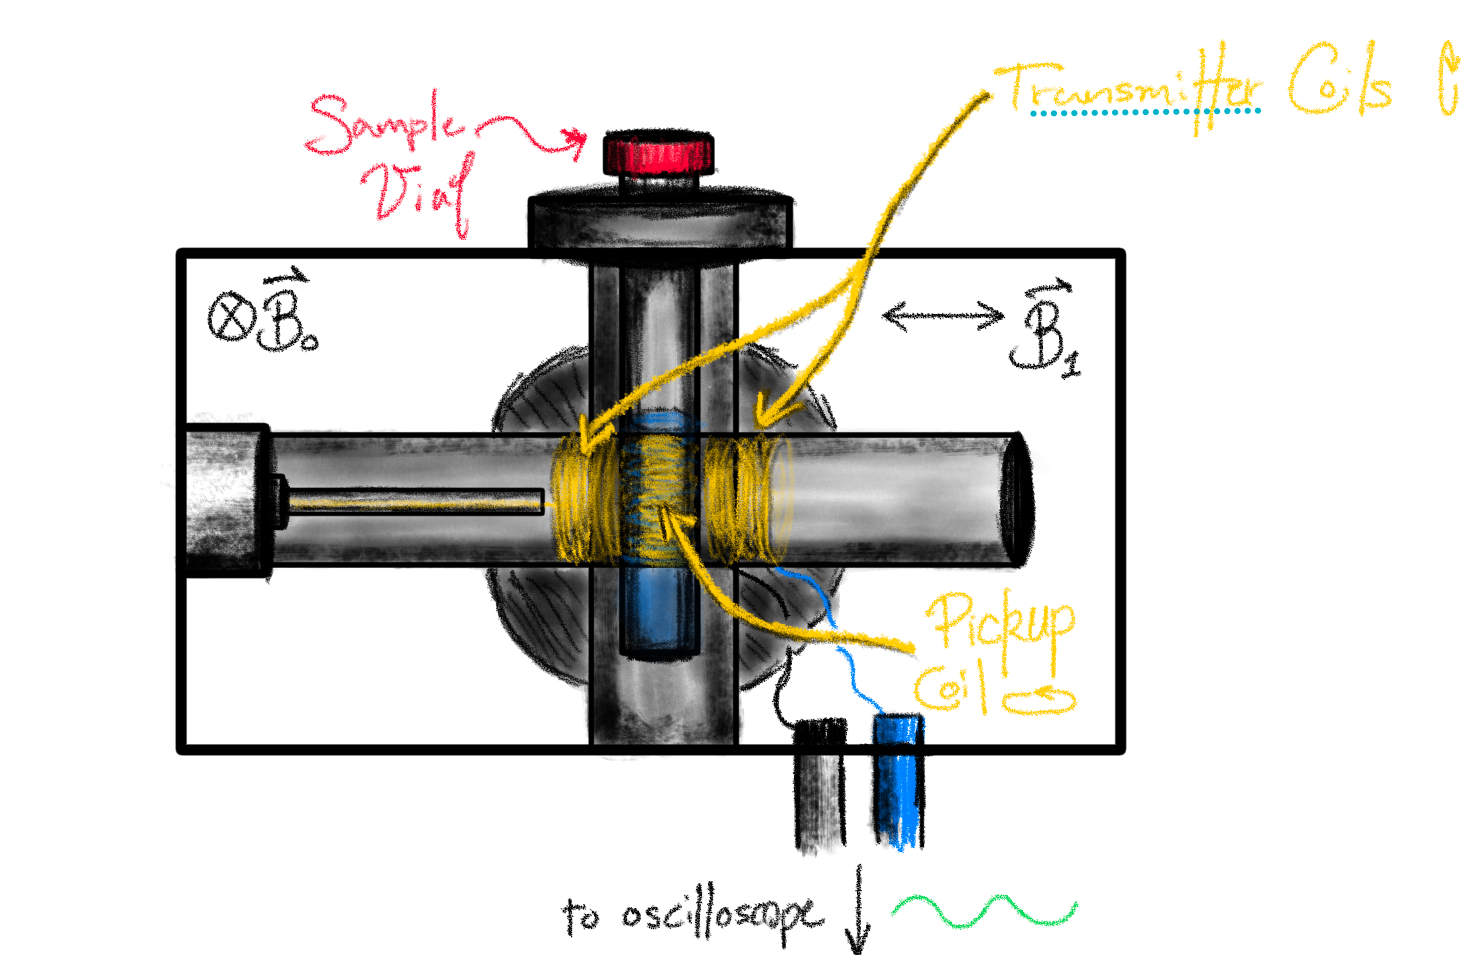
\includegraphics[width=6in]{5-nmr/overleaf/images/diagram.jpg}
        \caption{A sketched diagram of the experimental apparatus.}
        \label{fig:experiment-diagram}
    \end{figure}
    
    We measured the spin-lattice and spin–spin relaxation times ($T_1$ and $T_2$, respectively) of hydrogen in the non-polar molecules \textbf{glycerin} (\ce{C3H8O3}) and \textbf{mineral oil} (\ce{C16H10N2Na2O7S2}), conducting our observations using the TeachSpin\textsuperscript{\tiny\textregistered} \textsc{nmr} apparatus shown in \textbf{Figure~\ref{fig:experiment-diagram}}. After inserting the chosen sample, we initiated each experiment by calibrating the signal generator’s reference frequency to align with the receiver coil signal, adjusting for a minimum beat frequency on the oscilloscope’s second channel (using an appropriate zoom level) using the provided signal mixer (not pictured).

    In both \textsc{sl} and \textsc{ss} relaxation, we used a series of two pulses to manipulate the sample and isolate the chosen energy transfer pathway.
    \subsection*{Spin–Lattice Relaxation}
    {
        In the \textsc{sl} case, we adjusted the primary (A) pulse to be at an amplitude minimum and the secondary (B) pulse to be at an amplitude maximum. We varied the time interval $\Delta t$ between these two pulses from \SI{1}{\milli\second} to \SI{100}{\milli\second} in steps of \SI{1}{\milli\second}, using the oscilloscope cursors to measure a lower and upper bound for the amplitude (voltage) of the B pulse at each time step. We then plotted $V_{\mathrm{B}}(\Delta t)$ with offset removal and derectification, performing a regression fitting using \textbf{Equation~\ref{eq:1}} as the fit function. An optimal $T_1$ was determined with associated errors based on the fit.
    }
    \subsection*{Spin–Spin Relaxation}
    {
        In the \textsc{ss} case, we adjusted the primary (A) pulse to be at an amplitude maximum and the secondary (B) pulse to be at an amplitude minimum. In this case, a third echo pulse delayed from the B pulse by the same time interval $\Delta t$ was adjusted to a maximum as a proxy for minimizing the B pulse. We varied the time interval $\Delta t$ between these two pulses from \SI{1}{\milli\second} to $\sim$\SI{40}{\milli\second} in steps of \SI{1}{\milli\second}, using the oscilloscope cursors to measure a lower and upper bound for the amplitude (voltage) of the echo pulse at each time step. We then plotted $V_{\mathrm{echo}}(\Delta t)$ with debiasing and derectification, performing a regression fitting using \textbf{Equation~\ref{eq:1}} as the fit function. An optimal $T_1$ was determined with associated errors based on the fit.
    }

    \subsection*{Debiasing and Derectification}
    {
        In both cases, we observed rectification (loss of +/- parity) due to what is effectively a vector projection into the sensitive plane of the pickup coil. We lose sign information here because $\bm{\mu}$ can point along $+\hat{\mathrm{z}}$ or $-\hat{\mathrm{z}}$ and look the same to the pickup coil. In order to rectify this,\footnote{\textit{Ba dum tss.}} we wrote debiasing and derectification functions using \code{pandas}, which we applied respectively to each dataset prior to fitting.
    }
}

\section*{Results}
{
    Using the Python fitting package \code{scipy.optimize}, we performed regression fittings (\textbf{Figure~ \ref{fig:fit-plots}}) to find spin-lattice and spin–spin relaxation times ($T_1$ and $T_2$, respectively) of Hydrogen within the non-polar molecules \textbf{glycerin} (\ce{C3H8O3}) and \textbf{mineral oil} (\ce{C16H10N2Na2O7S2}), which are compiled in \textbf{Table\ \ref{tab:relaxation-times}.} 
}

\begin{figure}[tbh]
    \centering
    % First Row
    \begin{subfigure}{0.45\textwidth}
        \centering
        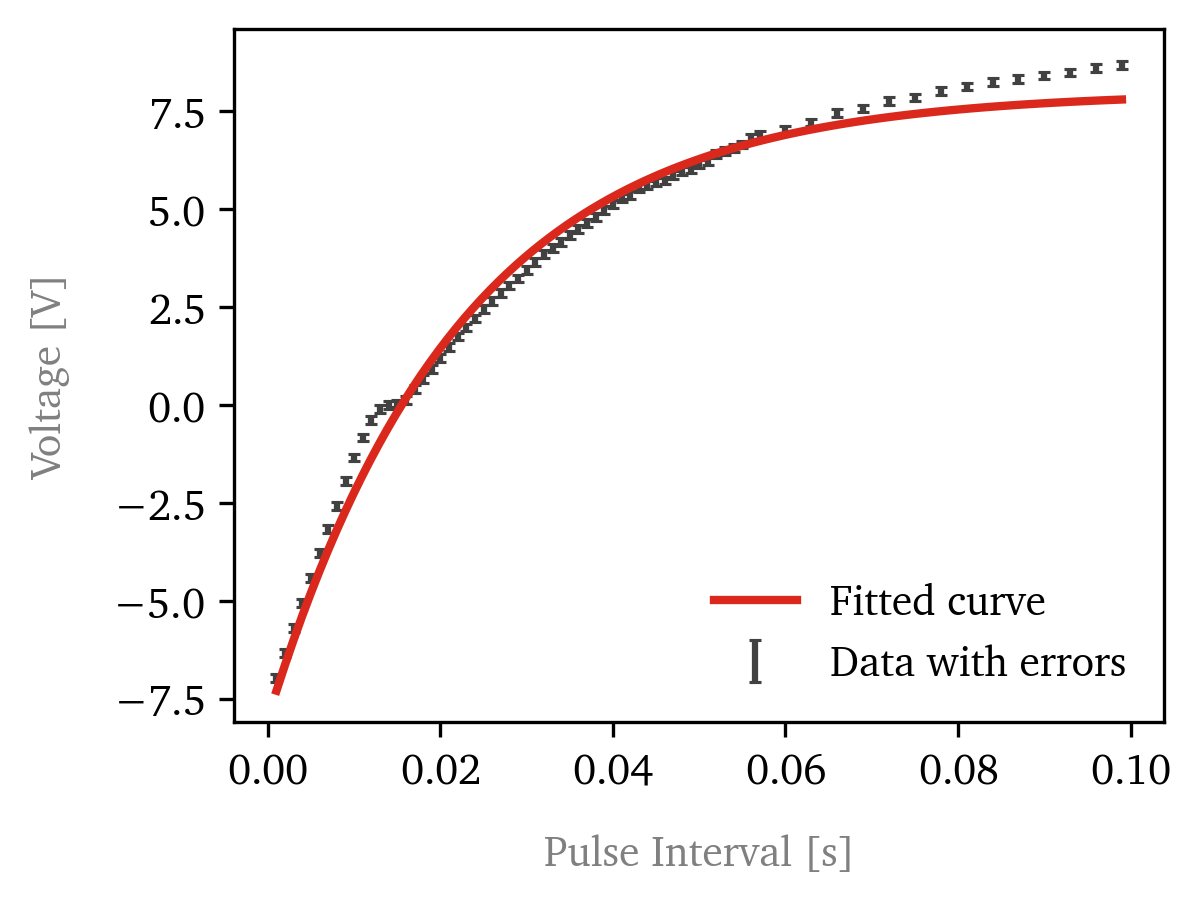
\includegraphics[width=\linewidth]{sl-glycerin.png}
        \caption{Spin–lattice (\textsc{sl}), glycerin.}
        \label{fig:sl-glycerin}
    \end{subfigure}
    \hspace{0.02\textwidth} % Reduced horizontal space between columns
    \begin{subfigure}{0.45\textwidth}
        \centering
        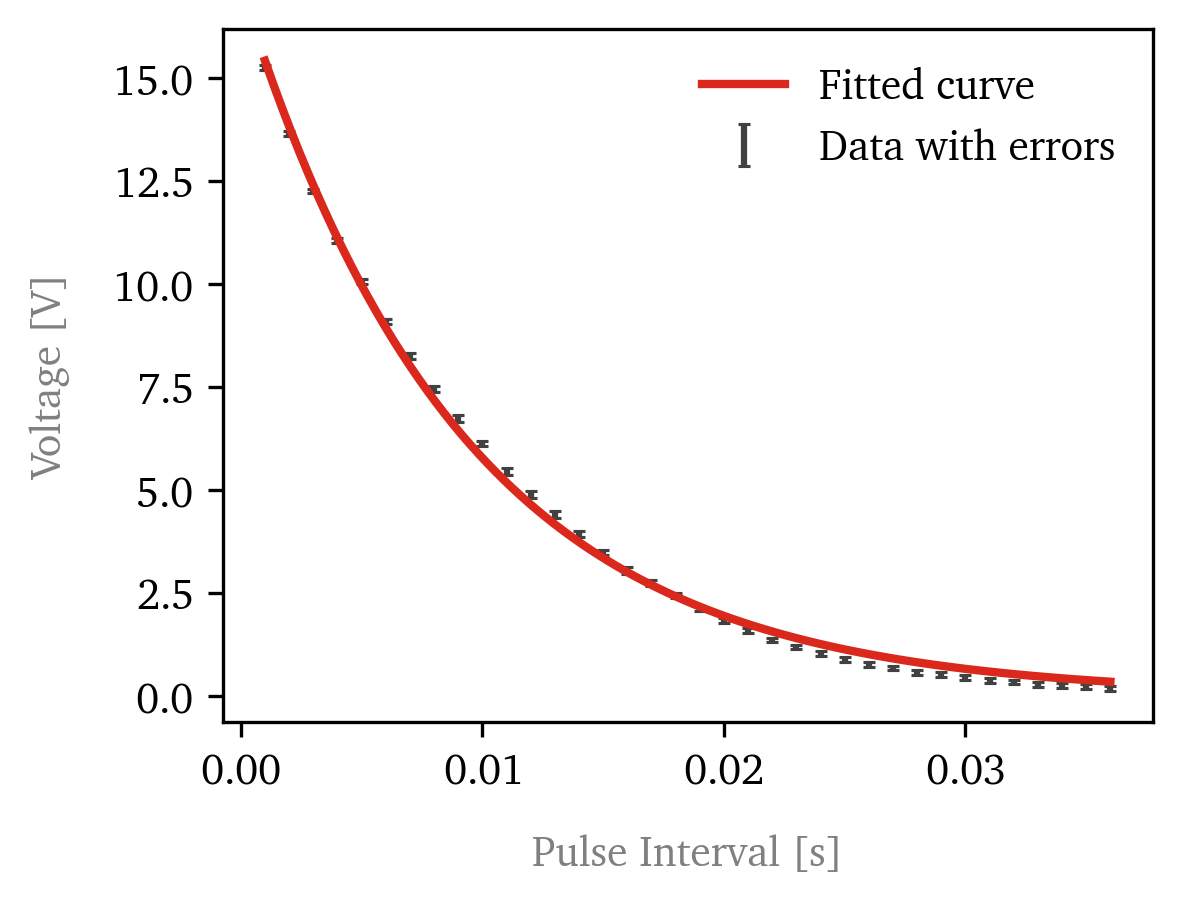
\includegraphics[width=\linewidth]{ss-glycerin.png}
        \caption{Spin–spin (\textsc{ss}), glycerin.}
        \label{fig:ss-glycerin}
    \end{subfigure}
    
    \vspace{\baselineskip} % Vertical space between rows
    
    % Second Row
    \begin{subfigure}{0.45\textwidth}
        \centering
        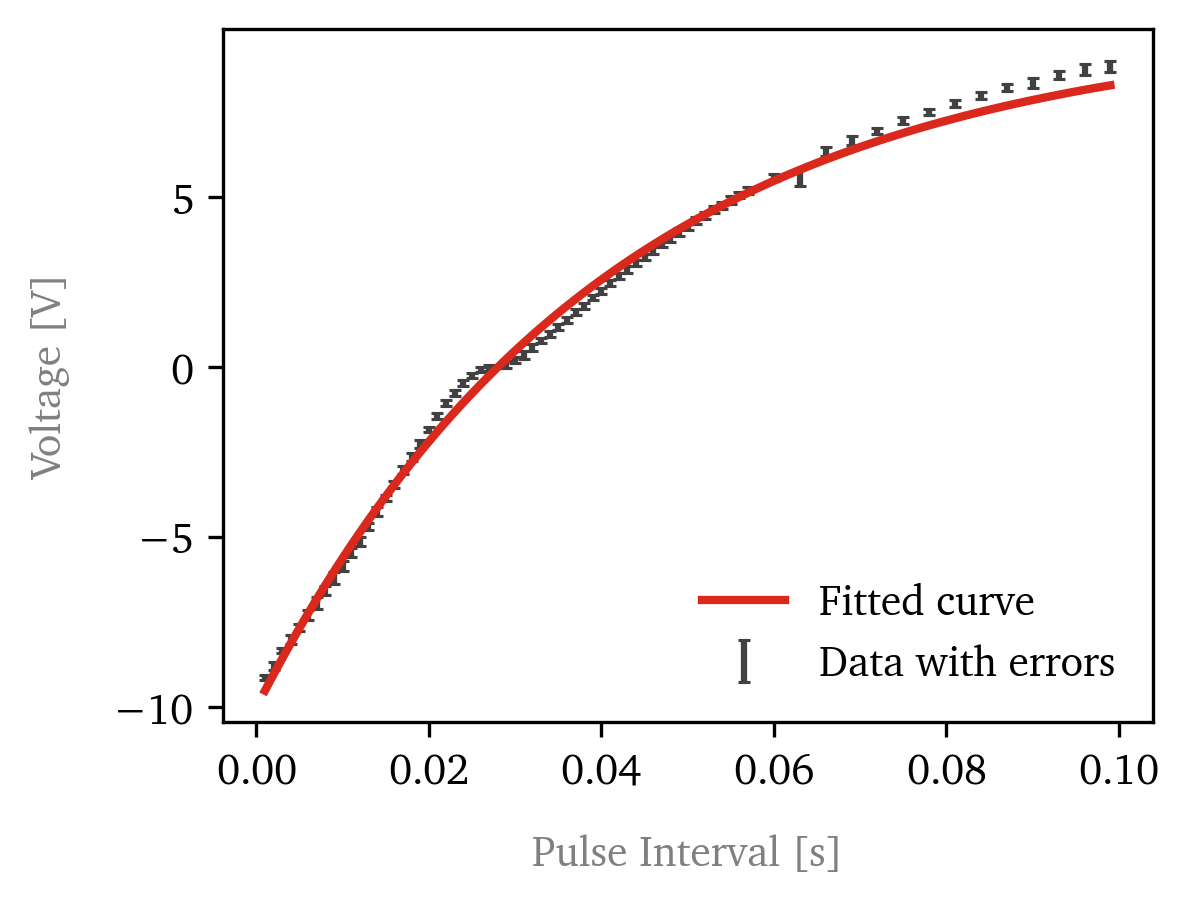
\includegraphics[width=\linewidth]{sl-mineral_oil.png}
        \caption{Spin–lattice (\textsc{sl}), mineral oil.}
        \label{fig:sl-mineral-oil}
    \end{subfigure}
    \hspace{0.02\textwidth} % Reduced horizontal space between columns
    \begin{subfigure}{0.45\textwidth}
        \centering
        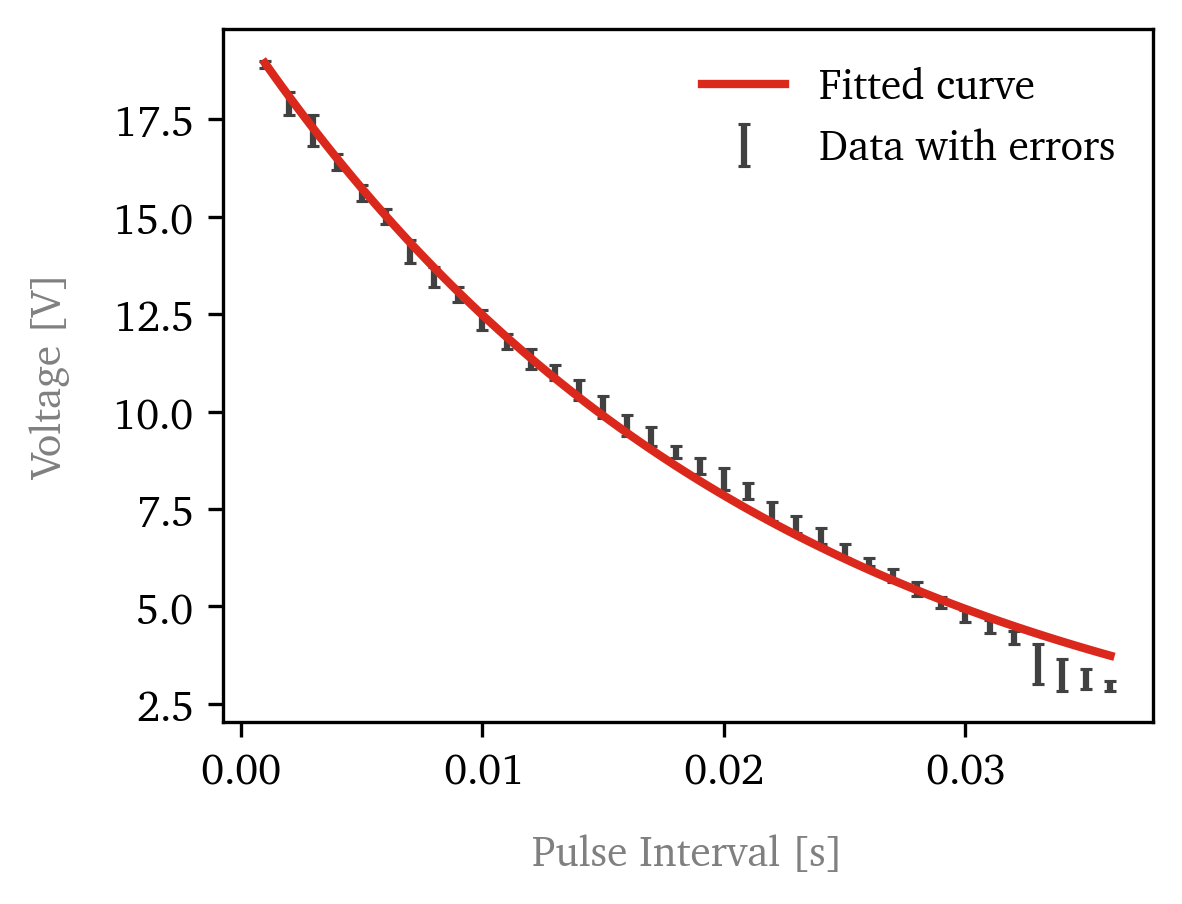
\includegraphics[width=\linewidth]{ss-mineral_oil.png}
        \caption{Spin–spin (\textsc{ss}), mineral oil.}
        \label{fig:ss-mineral-oil}
    \end{subfigure}
    
    \caption{Comparison of spin–lattice (\textsc{sl}) and spin–spin (\textsc{ss}) relaxation measurements for glycerin and mineral oil samples. Each plot shows the decay of voltage, $V$, versus the \textsc{rf} pulse interval, $\Delta t$. Best fit values for $T_1$ and $T_2$ are shown in \textbf{Table~\ref{tab:relaxation-times}}.}
    \label{fig:fit-plots}
\end{figure}

\begin{table}[tbh]
    \centering
    \begin{tabular}{rccc}
         \textbf{Material}   && $T_1$ (s) & $T_2$ (s) \\ \hline
        Glycerin    && $(2.21 \pm 0.03) \times 10^{-2}$ & $(8.55 \pm 1.52) \times 10^{-3}$ \\
        Mineral Oil && $(4.04 \pm 0.000\,000\,006) \times 10^{-2}$ & $(2.16 \pm 0.015) \times 10^{-2}$ \\
    \end{tabular}
    \caption{Relaxation times $T_1$ and $T_2$ for glycerin and mineral oil, with associated measurement errors. Associated fit plots are shown in \textbf{Figure~\ref{fig:fit-plots}}.}
    \label{tab:relaxation-times}
\end{table}


\end{document}